\documentclass[12pt,letterpaper, onecolumn]{exam}
\usepackage{amsmath}
\usepackage{amssymb}
\usepackage{commath}
\usepackage{physics}
\usepackage{multirow}
\usepackage{float}
\usepackage{relsize}
\usepackage{tikz}
\usepackage[lmargin=71pt, tmargin=1.2in]{geometry}  %For centering solution box
\usepackage{clrscode}
\usepackage{listings}
\usepackage{xcolor}
\usepackage{pdfpages}
\usepackage{enumitem}
\definecolor{codegreen}{rgb}{0,0.6,0}
\definecolor{codegray}{rgb}{0.5,0.5,0.5}
\definecolor{codepurple}{rgb}{0.58,0,0.82}
\definecolor{backcolour}{rgb}{0.95,0.95,0.92}
\usetikzlibrary{arrows.meta}
\usetikzlibrary{patterns}
\graphicspath{ {./images/} }

\lstdefinestyle{mystyle}{
    backgroundcolor=\color{backcolour},   
    commentstyle=\color{codegreen},
    keywordstyle=\color{magenta},
    numberstyle=\tiny\color{codegray},
    stringstyle=\color{codepurple},
    basicstyle=\ttfamily\footnotesize,
    breakatwhitespace=false,         
    breaklines=true,                 
    captionpos=b,                    
    keepspaces=true,                 
    numbers=left,                    
    numbersep=1pt,                  
    showspaces=false,                
    showstringspaces=false,
    showtabs=false,                  
    tabsize=2
}

%\lstset{style=mystyle}
\lhead{CAP 5610 Assignment \#3 Solution\\}
\rhead{Arman Sayan\\}
% \chead{\hline} % Un-comment to draw line below header
\thispagestyle{empty}   %For removing header/footer from page 1

\begin{document}

\begingroup  
    \centering
    \LARGE CAP 5610\\
    \LARGE Assignment \#3 Solution\\[0.5em]
    \large \today\\[0.5em]
    \large Arman Sayan\par
\endgroup
\rule{\textwidth}{0.4pt}
\bracketedpoints   %Self-explanatory
\printanswers
\renewcommand{\solutiontitle}{\noindent\textbf{Ans:}\enspace}   %Replace "Ans:" with starting keyword in solution box
\qformat{\large \textbf{\thequestion \quad \thequestiontitle \quad [\thepoints] \hfill}}
\renewcommand{\thepartno}{\arabic{partno}}
\renewcommand{\partlabel}{\thepartno.}

\begin{questions}
    \titledquestion{Kernel Computation Cost}[30]
    
    \begin{parts}
        \part[10]  Consider we have a two-dimensional input space such that the input vector is
        $x = (x_1, x_2)^T$. Define the feature mapping $\phi(x) = (x_1^2, \sqrt{2}x_1x_2, x_2^2)^T$. What is the corresponding
        kernel function, i.e., $K(x, z)$? Do not leave $\phi(x)$ in your final answer.

        \begin{solution}

            To find the kernel function $K(x, z)$, we use the definition of the kernel function as follows:

            \begin{equation*}
                K(x, z) = \phi(x)^T \phi(z)
            \end{equation*}

            where $\phi(x)$ represents feature mapping.

            Given that $\phi(x) = (x_1^2, \sqrt{2}x_1x_2, x_2^2)^T$, for another input vector $z = (z_1, z_2)^T$,
            the feature mapping is $\phi(z) = (z_1^2, \sqrt{2}z_1z_2, z_2^2)^T$.

            Now, we can compute the dot product of the feature mappings as follows:

            \begin{align*}
                K(x, z) &= \phi(x)^T \phi(z)\\ 
                &= \begin{bmatrix}
                    x_1^2 & \sqrt{2}x_1x_2 & x_2^2
                \end{bmatrix}
                \begin{bmatrix}
                    z_1^2\\
                    \sqrt{2}z_1z_2\\
                    z_2^2
                \end{bmatrix}\\
                &= x_1^2z_1^2 + 2x_1x_2z_1z_2 + x_2^2z_2^2\\
            \end{align*}

            With a deduction from the above calculations, we can observe the final expression as

            \begin{center}
                $K(x, z) = (x_1z_1 + x_2z_2)^2$
            \end{center}

            Since $x_1z_1 + x_2z_2$ is the dot product of the input vectors $x$ and $z$, namely $x^Tz$, 
            the corresponding kernel function is 

            \begin{center}
                \fbox{$\displaystyle{\boldsymbol{K(x, z) = (x^Tz)^2}}$}
            \end{center}

        \end{solution}

        \part[20] Suppose we want to compute the value of the kernel function $K(x, z)$ from the
        previous question on two vectors $x, z \in \mathbb{R}^2$. How many additions and multiplications are
        needed if you

        \begin{subparts}
            
            \subpart[10] Map the input vector to the feature space and then perform the dot product
            on the mapped features?

            \begin{solution}

                Using the feature mappings 
                
                \begin{center}
                    $\phi(x) = (x_1^2, \sqrt{2}x_1x_2, x_2^2)^T$ and $\phi(z) = (z_1^2, \sqrt{2}z_1z_2, z_2^2)^T$,
                \end{center}
                
                the kernel function $K(x, z)$ can be computed as

                \begin{align*}
                    K(x, z) &= \phi(x)^T \phi(z)\\ 
                    &= \begin{bmatrix}
                        x_1^2 & \sqrt{2}x_1x_2 & x_2^2
                    \end{bmatrix}
                    \begin{bmatrix}
                        z_1^2\\
                        \sqrt{2}z_1z_2\\
                        z_2^2
                    \end{bmatrix}\\
                    &= x_1^2z_1^2 + 2x_1x_2z_1z_2 + x_2^2z_2^2\\
                \end{align*}

                For the feature mapping of the vector $x$, we need to compute terms $x_1^2$, $x_2^2$, and $\sqrt{2}x_1x_2$.
                To calculate these terms, we need 3 multiplications.

                Since we have 2 input vectors $x$ and $z$, we need to perform 3 multiplications for each vector, which results in 6 multiplications
                for mapping the vectors to the feature space.

                After mapping the vectors to the feature space, we need to compute the dot product of the feature mappings as

                \begin{center}
                    $K(x, z) = x_1^2z_1^2 + 2x_1x_2z_1z_2 + x_2^2z_2^2$
                \end{center}

                This requires 3 multiplications for each term in the summation and 2 additions to sum three terms. 
                
                In total, we need \fbox{\textbf{9 multiplications and 2 additions}} to compute the value of $K(x, z)$.

            \end{solution}

            \pagebreak

            \subpart[10] Compute through the kernel function you derived in question 1?

            \begin{solution}

                The kernel function derived in question 1 is $K(x, z) = (x^Tz)^2$.

                To compute the value of the kernel function $K(x, z)$ using this kernel function, we need to calculate the dot product of the input vectors $x$ and $z$,
                namely $x^Tz$.

                The dot product of two vectors $x$ and $z$ is calculated as

                \begin{center}
                    $x^Tz = x_1z_1 + x_2z_2$
                \end{center}

                This requires 2 multiplications for terms $x_1z_1$ and $x_2z_2$ and 1 addition to sum those terms.

                After computing the dot product, we need to square the result to obtain the value of the kernel function $K(x, z)$.

                Squaring the result requires 1 multiplication.

                In total, we need \fbox{\textbf{3 multiplications and 1 addition}} to compute the value of $K(x, z)$.
                
            \end{solution}

        \end{subparts}

    \end{parts}

    \pagebreak

    \titledquestion{Activation Functions and Loss Functions}[30]

    \begin{parts}

        \part[20] For this assignment, you are encouraged to consult Dr. GOOGLE and Dr. ChatGPT. But please explain
        things in your own language while you write the answer. For each of the following activation functions,
        briefly describe the type of non-linearity (if any) it introduces and discuss their pros and cons.

        \begin{enumerate}[label=(\alph*)]
            \item Linear Activation Function
            \item Sigmoid Activation Function
            \item Tanh Activation Function
            \item ReLU (Rectified Linear Unit) Activation Function
        \end{enumerate}

        \begin{solution}

            \begin{enumerate}[label=(\alph*)]
                \item \textbf{Linear Activation Function:}
                
                \begin{center}
                    $f(x) = x$
                \end{center}

                Linear activation function introduces a linear relationship between the 
                input and output where the output is directly proportional to the input. 
                It is a simple activation function that does not introduce any 
                non-linearity to the model.

                It is simple and computationally efficient, making it useful for regression
                problems. However, it does not introduce any non-linearity, meaning it cannot 
                capture complex relationships in data, and stacking multiple linear layers does
                not increase the model’s learning capacity.
                
                \item \textbf{Sigmoid Activation Function:}
                
                \begin{center}
                    $f(x) = \dfrac{1}{1 + e^{-x}}$
                \end{center}

                Sigmoid activation function introduces a non-linearity that squashes the
                input values between 0 and 1 in a S-shaped curve. 
                
                It is useful for binary classification problems where the output is required
                to be in the range of 0 and 1. Furthermore, it provides a smooth gradient that
                helps in training the model. However, it suffers from the vanishing gradient
                problem, which makes training deep neural networks difficult. Also, it is not
                zero-centered, namely the output is always positive, which can lead to 
                convergence issues.

                \pagebreak
                
                \item \textbf{Tanh Activation Function:}
                
                \begin{center}
                    $f(x) = \dfrac{e^x - e^{-x}}{e^x + e^{-x}}$
                \end{center}

                Tanh activation function introduces a non-linearity that squashes the input
                values in a S-shaped curve, similar to sigmoid activation function, but output values 
                between -1 and 1.

                It is zero-centered, which helps in faster convergence during training.
                Also, it provides stronger gradients for hidden layers compared to sigmoid activation function.
                However, just like sigmoid activation function, it also suffers from the 
                vanishing gradient problem, making it difficult to train deep neural networks. 
                Furthermore, it is not suitable for sparse data. Lastly, it is computationally
                expensive due to the exponential operations.
                
                \item \textbf{ReLU (Rectified Linear Unit) Activation Function:}
                
                \begin{center}
                    $f(x) = \max(0, x)$
                \end{center}

                ReLU activation function introduces a non-linearity that outputs the input
                as it is if it is positive, and zero otherwise, making computations simple.
                
                It is computationally efficient and helps in faster convergence during training
                compared to sigmoid and tanh. Also, it does not suffer from the vanishing gradient
                problem, making it suitable for training deep neural networks. Lastly, it remains 
                one of the most widely used activation functions due to its strong performance 
                in deep networks. However, it suffers from the dying ReLU problem where neurons 
                can die during training and stop learning when inputs become negative and ReLU 
                outputs 0. Also, it is not zero-centered, which can lead to convergence issues.
                Lastly, it is not suitable for small input values as it ignores negative information.
                
            \end{enumerate}

        \end{solution}

        \pagebreak

        \part[10] For each of the following loss functions, briefly describe their mathematical formula and discuss for which type of
        learning task (classification, regression, etc.) they are most appropriate.

        \begin{enumerate}[label=(\alph*)]
            \item Mean Squared Error Loss
            \item Binary Cross Entropy Loss
            \item Hinge Loss
            \item Softmax Cross Entropy Loss
        \end{enumerate}

        \begin{solution}

            \begin{enumerate}[label=(\alph*)]
                \item \textbf{Mean Squared Error Loss:}
                
                Mean Squared Error (MSE) loss is a regression loss function that measures the average squared difference between the predicted values $\hat{y_i}$ and actual values $y_i$.
                
                \begin{center}
                    MSE $\displaystyle{= \dfrac{1}{N} \sum_{i=1}^{N} (y_i - \hat{y}_i)^2}$
                \end{center}

                where $N$ is the number of samples in the dataset, $y_i$ is the actual target value, and $\hat{y}_i$ is the predicted value.

                The squaring ensures that large errors are penalized more heavily than small errors.

                It is most appropriate for regression tasks where the model is required to predict continuous values.
                
                \item \textbf{Binary Cross Entropy Loss:}
                
                Binary Cross Entropy loss is a classification loss function that measures the difference between the predicted probability $\hat{y}_i$ and actual class labels for binary classification tasks.
                
                \begin{center}
                    BCE $\displaystyle{= -\dfrac{1}{N} \sum_{i=1}^{N} [y_i \log(\hat{y}_i) + (1 - y_i) \log(1 - \hat{y}_i)]}$
                \end{center}

                where $N$ is the number of samples in the dataset, $y_i$ is the actual class label such as 0 or 1, and $\hat{y}_i$ is the predicted probability between 0 and 1.

                The logarithm makes wrong confident predictions highly penalized.

                It is most appropriate for binary classification tasks where the model is required to predict probabilities for two classes. 
                
                \item \textbf{Hinge Loss:}
                
                Hinge loss is a classification loss function that measures the margin of the predicted class label $\hat{y}_i$ from the decision boundary for binary classification tasks.
                
                \begin{center}
                    Hinge Loss $\displaystyle{= \dfrac{1}{N} \sum_{i=1}^{N} \max(0, 1 - y_i \hat{y}_i)}$
                \end{center}

                where $N$ is the number of samples in the dataset, $y_i$ is the actual class label such as -1 or 1, and $\hat{y}_i$ is the predicted class label.

                If the true label $y_i$ and predicted label $\hat{y}_i$ have the same sign and a large margin greater than 1, the loss is 0.
                If that is not the case, it penalizes the prediction proportionally, encouraging a large decision margin between different classes.

                It is most appropriate for binary classification tasks where the model is required to predict class labels, like in SVMs.
                
                \item \textbf{Softmax Cross Entropy Loss:}
                
                Softmax Cross Entropy loss is a classification loss function that measures the difference between the predicted and actual class labels for multi-class classification
                tasks.

                \begin{center}
                    Softmax Cross Entropy $\displaystyle{= -\dfrac{1}{N} \sum_{i=1}^{N} \sum_{c=1}^{C} y_{i,c} \log(\frac{e^{\hat{y}_{i,c}}}{\sum_{k=1}^{C}{e^{\hat{y}_{i,k}}}})}$
                \end{center}

                where $N$ is the number of samples in the dataset, $C$ is the number of classes, $y_{i,c}$ is 1 if the true class is $c$ and 0 otherwise, and $\hat{y}_{i,c}$ is the raw predicted probability for class $c$
                before applying softmax.

                The softmax function converts raw model outputs into probabilities, and encourages high confidence in the correct class while penalizing incorrect ones.
                The cross-entropy term compares the predicted probability of the correct class to true label.

                It is most appropriate for multi-class classification tasks where each sample belongs to one of many classes and the model is required to predict probabilities for multiple classes.

            \end{enumerate}

        \end{solution}
        
    \end{parts}

    \pagebreak

    \titledquestion{Linear SVM Implementation}[40]

    Solution for Q3:

    \begin{solution}

        Please check the source codes and outputs included in the appendix named as

        \begin{center}
            \textbf{svm.py} and \textbf{SVM.ipynb} 
        \end{center}
        
        for the solution.
    \end{solution}

    \pagebreak
    
\end{questions}

\begin{appendix}
    \centering
    \begin{flushleft}  
      \section{Appendix}
      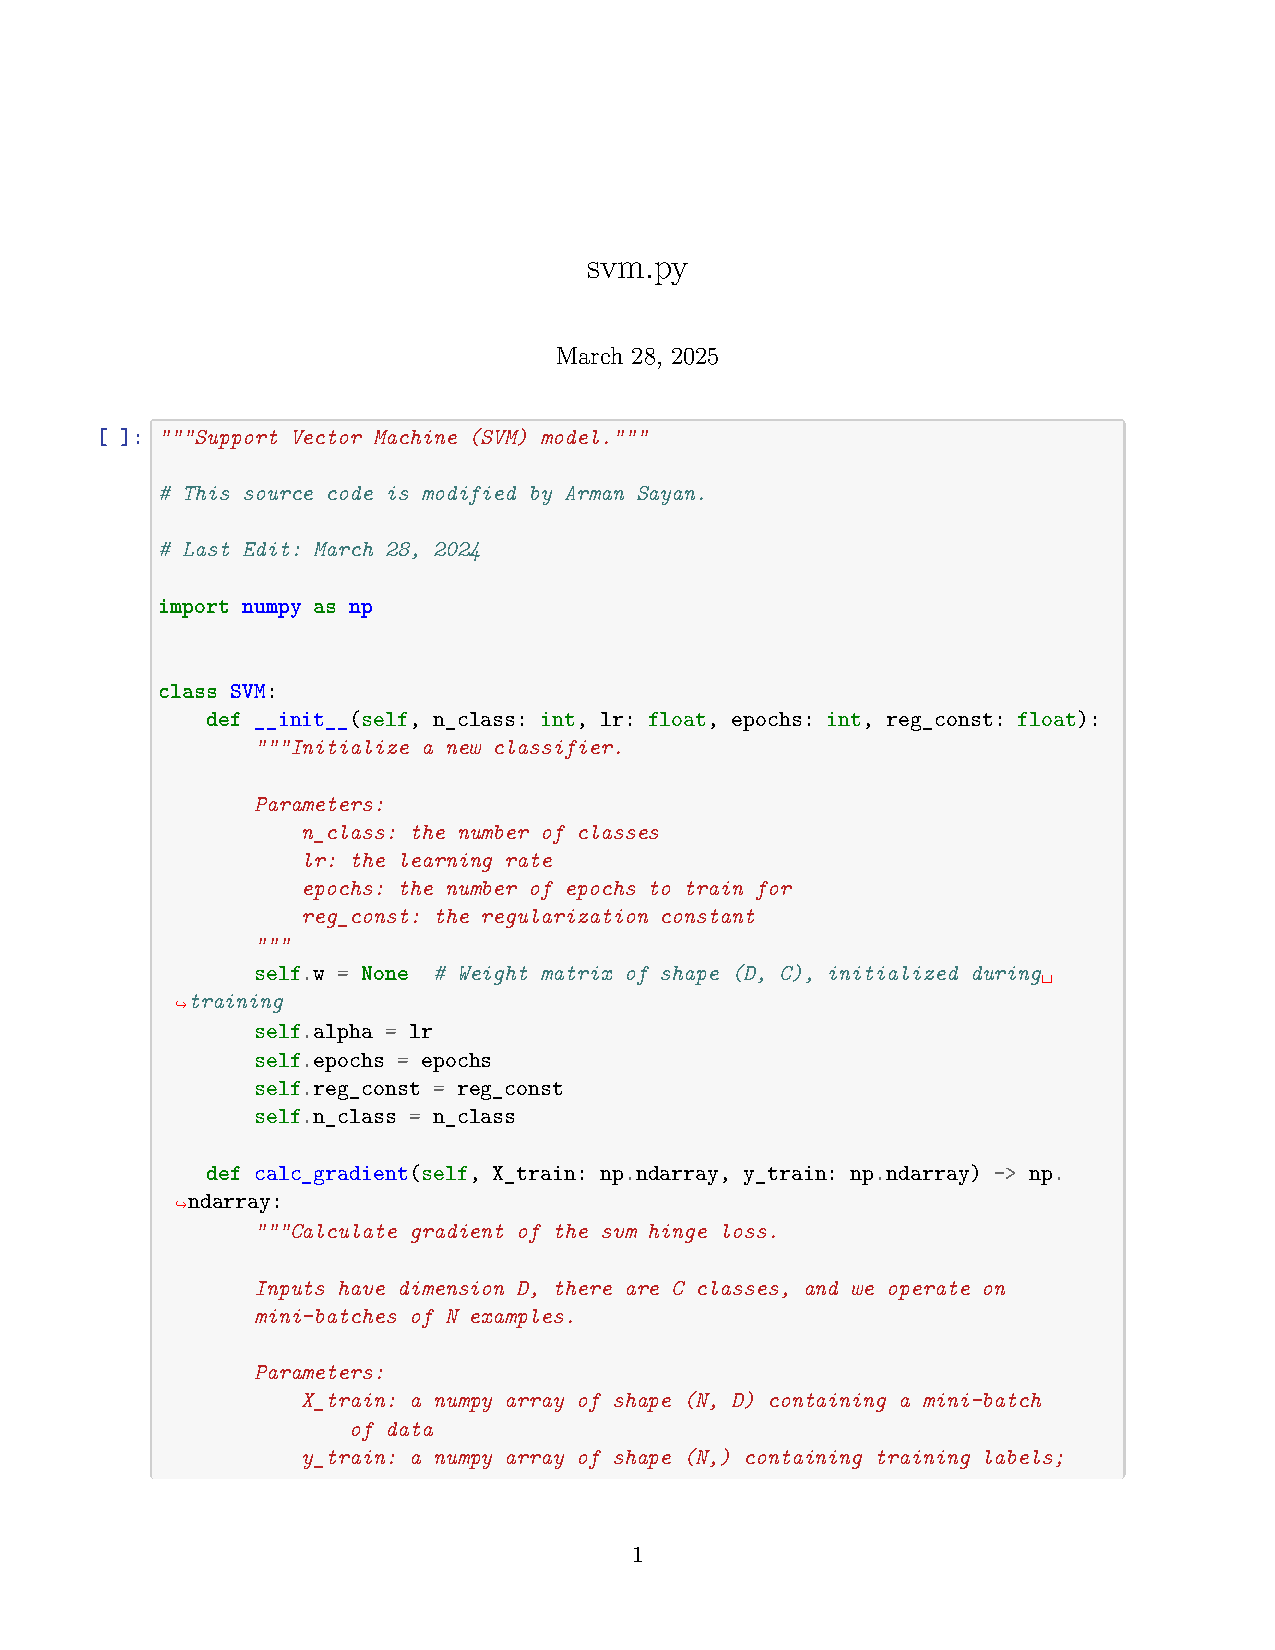
\includepdf[pages=-]{svm.py.pdf}
      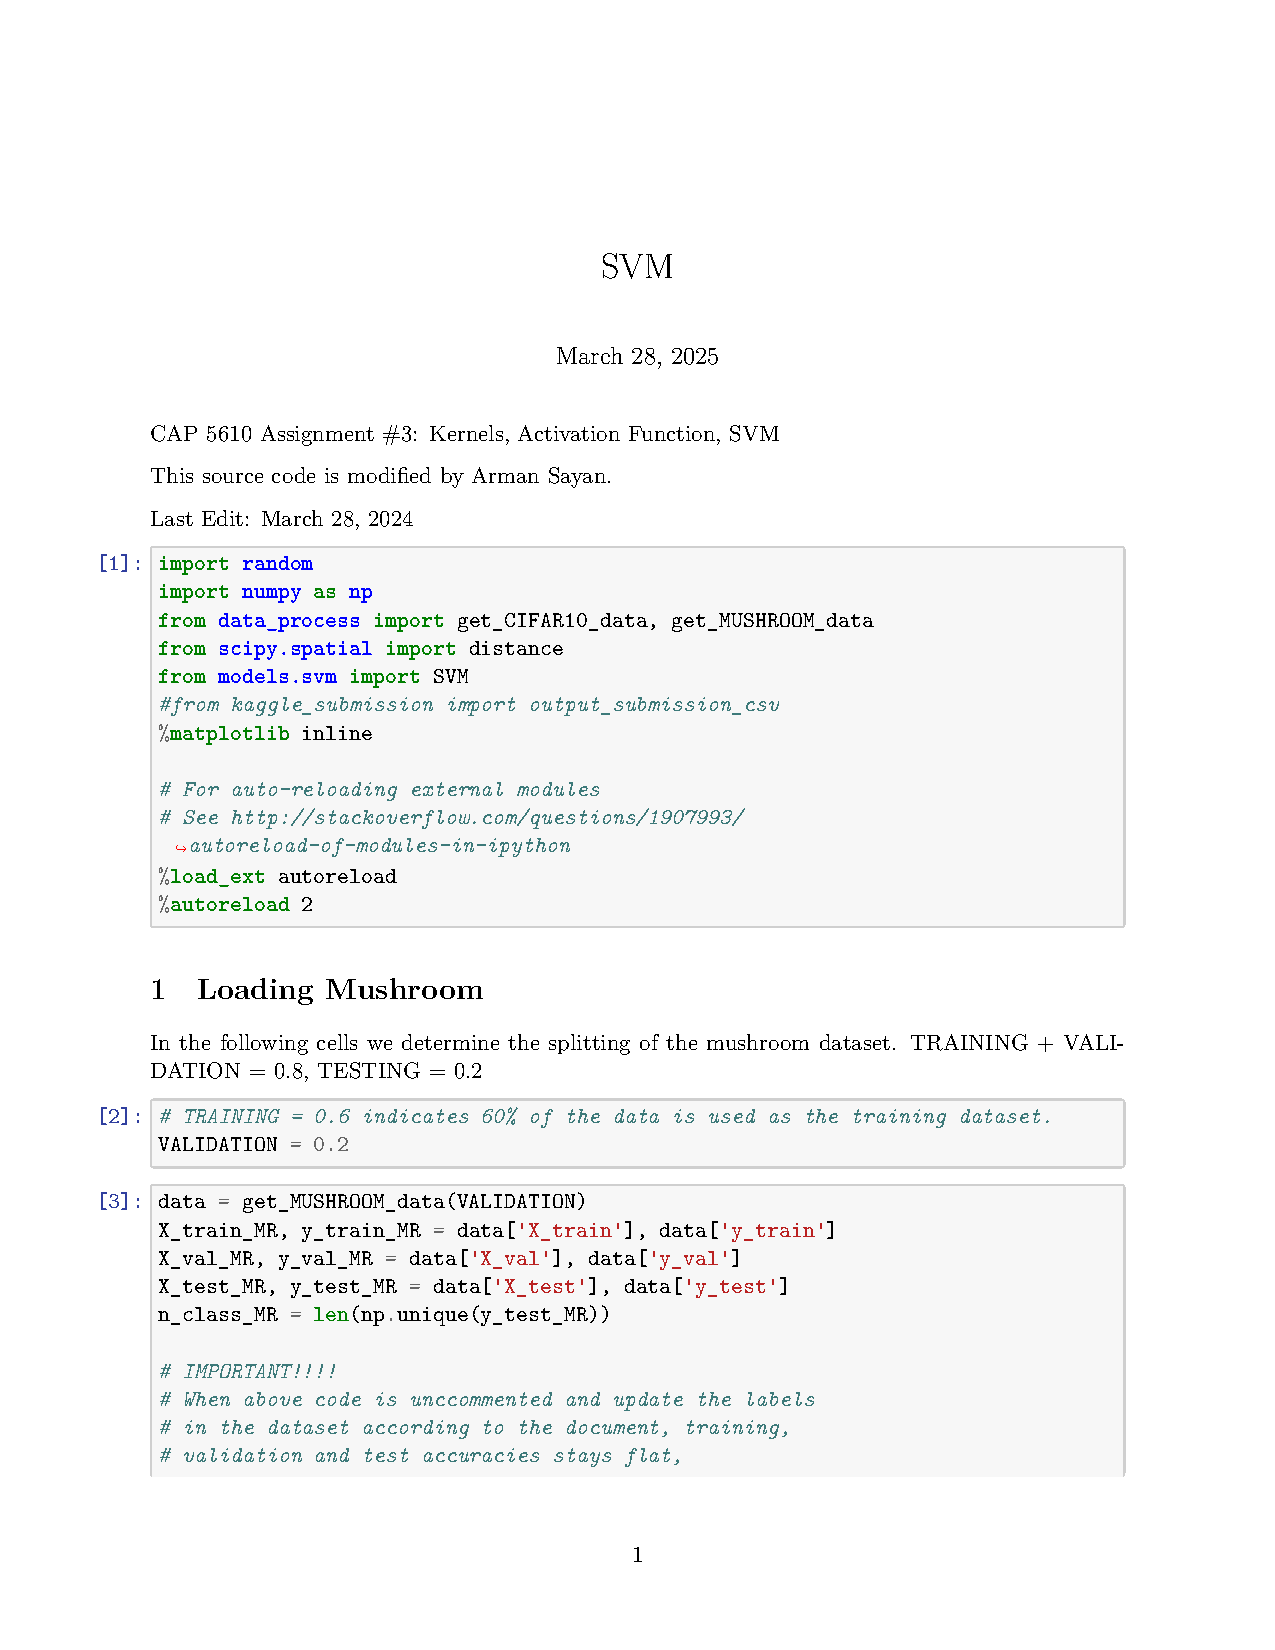
\includepdf[pages=-]{SVM_notebook.pdf}
    \end{flushleft}
\end{appendix}

\end{document}